% Options for packages loaded elsewhere
\PassOptionsToPackage{unicode}{hyperref}
\PassOptionsToPackage{hyphens}{url}
\PassOptionsToPackage{dvipsnames,svgnames,x11names}{xcolor}
%
\documentclass[
]{article}
\usepackage{amsmath,amssymb}
\usepackage{lmodern}
\usepackage{iftex}
\ifPDFTeX
  \usepackage[T1]{fontenc}
  \usepackage[utf8]{inputenc}
  \usepackage{textcomp} % provide euro and other symbols
\else % if luatex or xetex
  \usepackage{unicode-math}
  \defaultfontfeatures{Scale=MatchLowercase}
  \defaultfontfeatures[\rmfamily]{Ligatures=TeX,Scale=1}
  \setmainfont[]{Times New Roman}
  \setsansfont[]{JetBrains Mono}
\fi
% Use upquote if available, for straight quotes in verbatim environments
\IfFileExists{upquote.sty}{\usepackage{upquote}}{}
\IfFileExists{microtype.sty}{% use microtype if available
  \usepackage[]{microtype}
  \UseMicrotypeSet[protrusion]{basicmath} % disable protrusion for tt fonts
}{}
\usepackage{xcolor}
\usepackage[margin=1in]{geometry}
\usepackage{color}
\usepackage{fancyvrb}
\newcommand{\VerbBar}{|}
\newcommand{\VERB}{\Verb[commandchars=\\\{\}]}
\DefineVerbatimEnvironment{Highlighting}{Verbatim}{commandchars=\\\{\}}
% Add ',fontsize=\small' for more characters per line
\usepackage{framed}
\definecolor{shadecolor}{RGB}{248,248,248}
\newenvironment{Shaded}{\begin{snugshade}}{\end{snugshade}}
\newcommand{\AlertTok}[1]{\textcolor[rgb]{0.94,0.16,0.16}{#1}}
\newcommand{\AnnotationTok}[1]{\textcolor[rgb]{0.56,0.35,0.01}{\textbf{\textit{#1}}}}
\newcommand{\AttributeTok}[1]{\textcolor[rgb]{0.77,0.63,0.00}{#1}}
\newcommand{\BaseNTok}[1]{\textcolor[rgb]{0.00,0.00,0.81}{#1}}
\newcommand{\BuiltInTok}[1]{#1}
\newcommand{\CharTok}[1]{\textcolor[rgb]{0.31,0.60,0.02}{#1}}
\newcommand{\CommentTok}[1]{\textcolor[rgb]{0.56,0.35,0.01}{\textit{#1}}}
\newcommand{\CommentVarTok}[1]{\textcolor[rgb]{0.56,0.35,0.01}{\textbf{\textit{#1}}}}
\newcommand{\ConstantTok}[1]{\textcolor[rgb]{0.00,0.00,0.00}{#1}}
\newcommand{\ControlFlowTok}[1]{\textcolor[rgb]{0.13,0.29,0.53}{\textbf{#1}}}
\newcommand{\DataTypeTok}[1]{\textcolor[rgb]{0.13,0.29,0.53}{#1}}
\newcommand{\DecValTok}[1]{\textcolor[rgb]{0.00,0.00,0.81}{#1}}
\newcommand{\DocumentationTok}[1]{\textcolor[rgb]{0.56,0.35,0.01}{\textbf{\textit{#1}}}}
\newcommand{\ErrorTok}[1]{\textcolor[rgb]{0.64,0.00,0.00}{\textbf{#1}}}
\newcommand{\ExtensionTok}[1]{#1}
\newcommand{\FloatTok}[1]{\textcolor[rgb]{0.00,0.00,0.81}{#1}}
\newcommand{\FunctionTok}[1]{\textcolor[rgb]{0.00,0.00,0.00}{#1}}
\newcommand{\ImportTok}[1]{#1}
\newcommand{\InformationTok}[1]{\textcolor[rgb]{0.56,0.35,0.01}{\textbf{\textit{#1}}}}
\newcommand{\KeywordTok}[1]{\textcolor[rgb]{0.13,0.29,0.53}{\textbf{#1}}}
\newcommand{\NormalTok}[1]{#1}
\newcommand{\OperatorTok}[1]{\textcolor[rgb]{0.81,0.36,0.00}{\textbf{#1}}}
\newcommand{\OtherTok}[1]{\textcolor[rgb]{0.56,0.35,0.01}{#1}}
\newcommand{\PreprocessorTok}[1]{\textcolor[rgb]{0.56,0.35,0.01}{\textit{#1}}}
\newcommand{\RegionMarkerTok}[1]{#1}
\newcommand{\SpecialCharTok}[1]{\textcolor[rgb]{0.00,0.00,0.00}{#1}}
\newcommand{\SpecialStringTok}[1]{\textcolor[rgb]{0.31,0.60,0.02}{#1}}
\newcommand{\StringTok}[1]{\textcolor[rgb]{0.31,0.60,0.02}{#1}}
\newcommand{\VariableTok}[1]{\textcolor[rgb]{0.00,0.00,0.00}{#1}}
\newcommand{\VerbatimStringTok}[1]{\textcolor[rgb]{0.31,0.60,0.02}{#1}}
\newcommand{\WarningTok}[1]{\textcolor[rgb]{0.56,0.35,0.01}{\textbf{\textit{#1}}}}
\usepackage{longtable,booktabs,array}
\usepackage{calc} % for calculating minipage widths
% Correct order of tables after \paragraph or \subparagraph
\usepackage{etoolbox}
\makeatletter
\patchcmd\longtable{\par}{\if@noskipsec\mbox{}\fi\par}{}{}
\makeatother
% Allow footnotes in longtable head/foot
\IfFileExists{footnotehyper.sty}{\usepackage{footnotehyper}}{\usepackage{footnote}}
\makesavenoteenv{longtable}
\usepackage{graphicx}
\makeatletter
\def\maxwidth{\ifdim\Gin@nat@width>\linewidth\linewidth\else\Gin@nat@width\fi}
\def\maxheight{\ifdim\Gin@nat@height>\textheight\textheight\else\Gin@nat@height\fi}
\makeatother
% Scale images if necessary, so that they will not overflow the page
% margins by default, and it is still possible to overwrite the defaults
% using explicit options in \includegraphics[width, height, ...]{}
\setkeys{Gin}{width=\maxwidth,height=\maxheight,keepaspectratio}
% Set default figure placement to htbp
\makeatletter
\def\fps@figure{htbp}
\makeatother
\setlength{\emergencystretch}{3em} % prevent overfull lines
\providecommand{\tightlist}{%
  \setlength{\itemsep}{0pt}\setlength{\parskip}{0pt}}
\setcounter{secnumdepth}{5}
\newlength{\cslhangindent}
\setlength{\cslhangindent}{1.5em}
\newlength{\csllabelwidth}
\setlength{\csllabelwidth}{3em}
\newlength{\cslentryspacingunit} % times entry-spacing
\setlength{\cslentryspacingunit}{\parskip}
\newenvironment{CSLReferences}[2] % #1 hanging-ident, #2 entry spacing
 {% don't indent paragraphs
  \setlength{\parindent}{0pt}
  % turn on hanging indent if param 1 is 1
  \ifodd #1
  \let\oldpar\par
  \def\par{\hangindent=\cslhangindent\oldpar}
  \fi
  % set entry spacing
  \setlength{\parskip}{#2\cslentryspacingunit}
 }%
 {}
\usepackage{calc}
\newcommand{\CSLBlock}[1]{#1\hfill\break}
\newcommand{\CSLLeftMargin}[1]{\parbox[t]{\csllabelwidth}{#1}}
\newcommand{\CSLRightInline}[1]{\parbox[t]{\linewidth - \csllabelwidth}{#1}\break}
\newcommand{\CSLIndent}[1]{\hspace{\cslhangindent}#1}
% Line spacing
\renewcommand{\baselinestretch}{1.3}

% Page number and chapter at the top of the page
\pagestyle{headings}

% Important packages
\usepackage[utf8]{inputenc}
\usepackage[T1]{fontenc}
% \usepackage[dvipsnames]{xcolor}
\usepackage{hyperref}
\usepackage{dcolumn}
\usepackage{booktabs}
\usepackage{longtable}


% Figure and table names 
\usepackage{caption}
\captionsetup[table]{name=Tableau} 
\captionsetup[figure]{name=Figure}

% Packages for kableExtra
\usepackage{array}
\usepackage{multirow}
\usepackage{wrapfig}
\usepackage{colortbl}
\usepackage{pdflscape}
\usepackage{float}
\usepackage{tabu}
\usepackage{threeparttable}
\usepackage{threeparttablex}
\usepackage[normalem]{ulem}
\usepackage{makecell}

% Remove page numbering before start of redaction
\pagenumbering{gobble}

% Command to make a blank page
\usepackage{afterpage}
\newcommand\blankpage{%
    \null
    \thispagestyle{empty}%
    \addtocounter{page}{-1}%
    }
\usepackage{amsmath}
\ifLuaTeX
  \usepackage{selnolig}  % disable illegal ligatures
\fi
\IfFileExists{bookmark.sty}{\usepackage{bookmark}}{\usepackage{hyperref}}
\IfFileExists{xurl.sty}{\usepackage{xurl}}{} % add URL line breaks if available
\urlstyle{same} % disable monospaced font for URLs
\hypersetup{
  colorlinks=true,
  linkcolor={Maroon},
  filecolor={Maroon},
  citecolor={Blue},
  urlcolor={blue},
  pdfcreator={LaTeX via pandoc}}

\author{}
\date{\vspace{-2.5em}}

\begin{document}

\begin{titlepage}
\centering

\topskip0pt
\vspace*{\fill}
  {\Huge Creating Reproducible Environments with Nix for Scientific Computing}
\newline
\newline
Morphy Kuffour 

\href{mailto:morphy.kuffour@uconn.edu}{morphy.kuffour@uconn.edu}

Department of Computer Science and Engingeering, University of Connecticut

Thesis Advisor: Prof. Clay Tabor

Honors Advisor: Prof. Caiwen Ding
\vspace*{\fill}

\afterpage{\blankpage}
\end{titlepage}

\topskip0pt
\vspace*{\fill}
\begin{center}
  {\large \textbf{Abstract}}
\end{center}
The Nix package manager provides a way to manage dependencies between multiple software packages and configurations, enabling users to access various versions of a package and its dependencies. This allows users to maintain reproducible environments for the Community Earth System Model Version 2.0 (CESM 2.0) code across different platforms, specifically for its computational components, enabling developers to have a consistent development environment for scientific computing. Managed environments also provide a way for users to easily access and install new packages specific to the CESM project, as well as quickly update its existing packages. Using the nix package manager for reproducible development environments helps ensure accurate and consistent CESM project results, and makes it easier for developers to collaborate on the same project.
\vspace*{\fill}

\pagebreak

\pagenumbering{arabic}

\hypertarget{introduction}{%
\section{Introduction}\label{introduction}}

Scientific computing has become increasingly important in many fields of research, including physics, chemistry, biology, and Earth science. These fields rely heavily on complex software and tools to create, analyze, and visualize data. However, managing software dependencies and configurations across different platforms and systems can be challenging, and inconsistencies in these environments can lead to irreproducible results. This is where the nix package manager comes in to provide a solution.

The nix package manager provides a way to manage dependencies between multiple software packages and configurations, enabling users to access various versions of a package and its dependencies. This allows users to maintain reproducible environments for scientific computing across different platforms, enabling developers to have a consistent development environment for their projects. In particular, nix has proven to be a valuable tool for the CESM project, which is a complex modeling framework used to simulate the Earth's climate system.

In this paper, we will explore how the nix package manager can be used to create reproducible environments for scientific computing, with a focus on the CESM project. I will discuss the benefits of using nix for managing dependencies, how to create and manage nix environments, and share our experiences using nix for porting CESM project to the UConn High Performance Computing (HPC) system. I will also discuss the community support and resources available for nix users, and provide examples of other scientific computing projects that have successfully implemented nix for reproducibility. This paper aims to provide a comprehensive understanding of how nix facilitates reproducibility in scientific computing and offers guidance on incorporating nix into individual projects.

\hypertarget{need-for-software-reproducibility-in-scientific-computing}{%
\subsection{Need for software reproducibility in scientific computing}\label{need-for-software-reproducibility-in-scientific-computing}}

The need for software reproducibility in scientific computing cannot be overstated. Scientific research relies heavily on computer simulations and models to test hypotheses and make predictions. These simulations and models are typically implemented using various software packages and tools, and the results obtained from them are highly dependent on the specific versions of the software used, as well as the configurations and dependencies of the underlying systems.

In their paper titled ``Reproducibility in Scientific Computing'' (\protect\hyperlink{ref-reproduce0}{Ivie and Thain 2018}) provide a comprehensive analysis of the current state of reproducibility in computational research and highlight the urgent need for improving the reproducibility of scientific results. They argue that software is a critical component of scientific research and that the inability to reproduce scientific results due to software issues undermines the integrity and reliability of scientific research.

Furthermore, the lack of reproducibility can have significant consequences, both for the scientific community and for society at large. Incorrect or unverifiable scientific results can lead to misguided policies and decisions, wasting valuable resources and potentially endangering public health and safety. For instance, public distrust of climate science has resulted in a failure to act on the overwhelming evidence of anthropogenic climate change, leading to catastrophic consequences. Therefore, it is essential that scientific software be designed and developed in a way that ensures reproducibility and facilitates the sharing and reuse of scientific code.

To address the need for software reproducibility in scientific computing, various approaches and tools have been proposed, including containerization technologies like Docker and virtualization platforms like VirtualBox, as well as package managers like Nix, which enable the management of software dependencies and configurations. These tools and approaches help ensure that the software used in scientific research is fully documented and can be easily reproduced, validated, and reused by other researchers.

\hypertarget{nix-fundamentals}{%
\section{Nix Fundamentals}\label{nix-fundamentals}}

\hypertarget{introduction-to-nix}{%
\subsection{Introduction to Nix}\label{introduction-to-nix}}

Nix is a powerful package manager that provides a unique approach to dependency management and enables the creation of reproducible software environments. Unlike traditional package managers that rely on global installation and modification of system-level libraries, Nix uses a purely functional approach that ensures each package and its dependencies are installed in a self-contained and isolated environment. This allows for multiple versions of the same package to coexist on a system without interfering with each other. Moreover, Nix provides a declarative language for defining package dependencies and their configurations, which can be versioned and shared across different systems. By using Nix, developers can easily reproduce the exact same environment and dependencies needed to run an application, regardless of the host operating system and hardware. As a result, Nix has become a popular tool for creating reproducible environments in scientific computing, enabling researchers to easily share their work and reproduce their experiments on different platforms (\protect\hyperlink{ref-dolstra2004nix}{Dolstra et al. 2004}).

\hypertarget{nixs-approach-to-package-management}{%
\subsection{Nix's approach to package management}\label{nixs-approach-to-package-management}}

Nix provides a unique approach to package management compared to other traditional package managers. Instead of relying on a global installation location and modifying the system environment, Nix uses a purely functional approach to package management (\protect\hyperlink{ref-dolstra2004nix}{Dolstra et al. 2004}). Each package is installed into its own isolated environment, ensuring that packages do not interfere with each other and that dependencies are always satisfied. Additionally, Nix enables users to install multiple versions of the same package side-by-side, which can be useful for developers who need to test their software with different versions of a dependency.

Nix relies on a few essential components to implement its functional approach to package management. First, Nix uses a lazy evaluation model, meaning that packages are not built until they are needed. This allows Nix to build only the packages that are actually required, reducing the amount of unnecessary builds and saving disk space. Second, Nix uses a content-addressed store, where each package is stored with a unique content-based identifier. This means that if two packages have the same contents, they will share the same identifier and only be stored once, further reducing disk space usage. Finally, Nix uses the Nix expression language, which is a declarative language for describing packages and their dependencies.

Devresse et al.~(2015) note that Nix's approach to package management is distinct in that every package is immutable and the outcome of a stateless function, rendering it deterministic and idempotent for a particular set of inputs. This is accomplished through the application of SHA-256 binary hashes for each package, which are deposited and extracted from a centralized store implementing a Key-Value store model. As stated in the paper, ``In Nix, each package is immutable and the result of a stateless function, pure in the functional sense that is guaranteed to be deterministic and idempotent for a given set of inputs'' (\protect\hyperlink{ref-devresse2015nix}{Devresse, Delalondre, and Schürmann 2015}).

\begin{figure}
   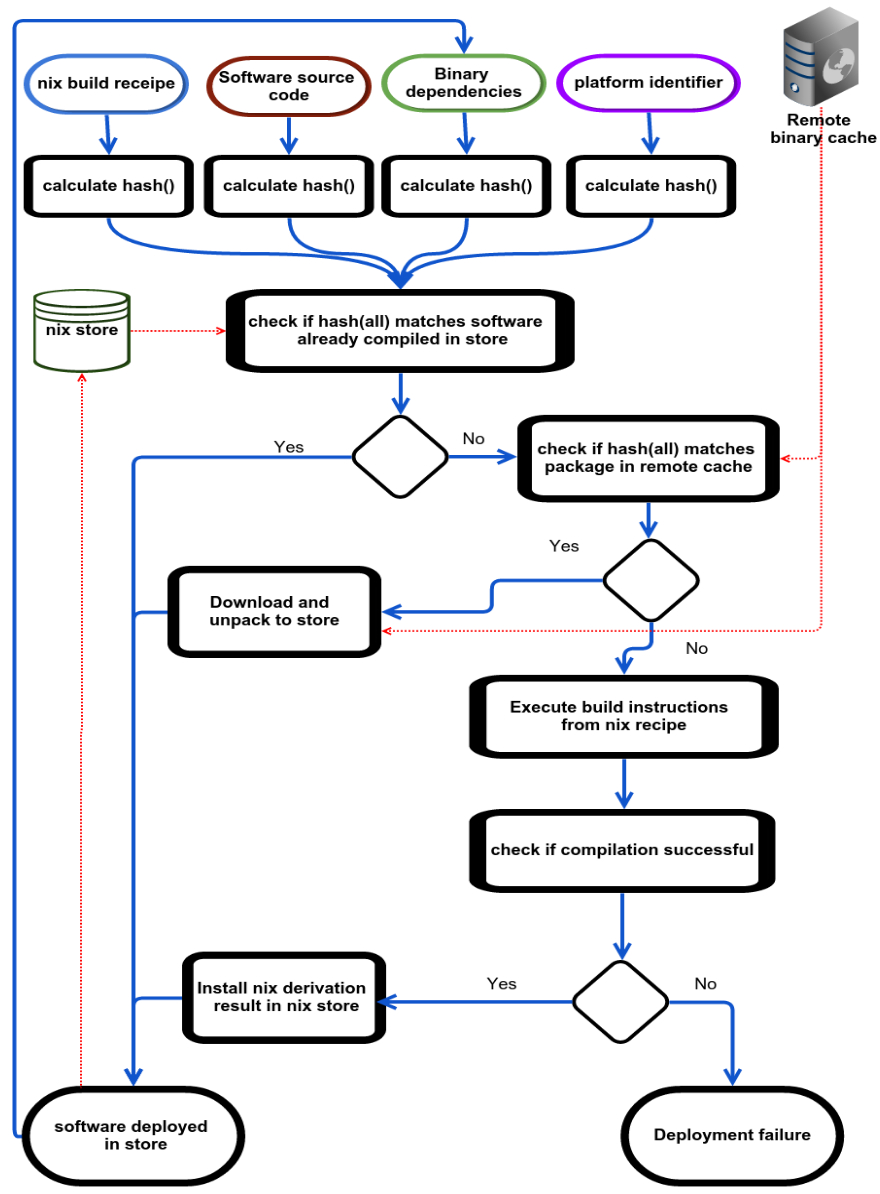
\includegraphics{./imgs/deps.png}
   \caption{A diagrammatic view of the process by which nix packages software and its dependencies}
   \label{fig:fig1}
\end{figure}

\hypertarget{related-work-nix-for-scientific-computing-management}{%
\section{Related Work: Nix for Scientific Computing Management}\label{related-work-nix-for-scientific-computing-management}}

Bzeznik et al.~(2017) discuss the challenges of using traditional package management systems on HPC clusters and how Nix can be used to overcome these challenges. It provides an overview of Nix and explains how it can be used to manage packages on HPC clusters (\protect\hyperlink{ref-bzeznik2017nix}{Bzeznik et al. 2017}).

The authors also present a case study of using Nix on a large HPC cluster at the University of Oslo. They demonstrate how Nix was used to manage packages and dependencies, resulting in a more streamlined and efficient package management system.

Overall, the paper provides valuable insights into the use of Nix on HPC clusters and highlights the advantages of using a functional package management system in this context. It can serve as a useful reference for researchers and system administrators looking to improve package management on HPC clusters.

\hypertarget{deploying-cesm-on-an-hpc-system-using-nix-package-manager}{%
\subsection{Deploying CESM on an HPC System Using Nix Package Manager}\label{deploying-cesm-on-an-hpc-system-using-nix-package-manager}}

CESM 2.1 is a complex and powerful software tool that allows researchers to simulate and study the Earth's climate. Deploying this tool to a high-performance computing (HPC) environment like the UConn HPC can be a daunting task, as it requires managing many dependencies and ensuring that the software is compiled and configured correctly.

During my work with Assistant Professor Clay Tabor, we utilized the Nix package manager to help facilitate the deployment of CESM to the UConn HPC. Nix allowed us to define a reproducible environment that included all the necessary dependencies for CESM, ensuring that the software was compiled and configured consistently across different runs and different systems.

Furthermore, Nix provided us with the ability to easily manage the many dependencies required by CESM, including complex scientific libraries like NetCDF and MPI. With Nix, we could easily define and manage the versions of these dependencies, ensuring that the correct versions were used for each run of the CESM model.

\hypertarget{building-and-managing-scientific-packages-with-nix}{%
\subsection{Building and managing scientific packages with Nix}\label{building-and-managing-scientific-packages-with-nix}}

Access to high-performance computing (HPC) systems is often limited, and users may have only limited sudo access, which can make installing and managing software a challenge. In our work deploying CESM to the UConn HPC, we encountered these limitations, but we were able to overcome them with the help of community software, such as nix-user-chroot.

Nix-user-chroot is a tool that allows users to create a Nix environment inside a chrooted directory, without requiring root access. This is particularly useful for HPC systems where users may not have sudo access. By using nix-user-chroot, we were able to create a self-contained environment for our CESM installation, with all of the required dependencies and configurations.

When working on deploying CESM to the UConn HPC, we encountered a challenge with limited sudo access to the HPC, which meant that we could not install new software or access software outside of the pre-installed HPC module.

With limited sudo access on an HPC, it was challenging to manage software dependencies and versions. The HPC may have specific software modules installed, but they may not be the required version or have the necessary dependencies. Additionally, installing software locally without sudo access can result in conflicting dependencies and installations, leading to a broken environment.

However, with the help of the community software nix-user-chroot, we were able to create a separate namespace environment with its own software dependencies and configurations. This allowed us to install and use the necessary software for CESM without interfering with the HPC module. The namespace separation provided by nix-user-chroot created an isolated environment where the necessary software packages could be installed and configured independently of the HPC module.

\hypertarget{disadvantages-of-using-nix-for-scientific-computing}{%
\subsection{Disadvantages of using Nix for Scientific Computing}\label{disadvantages-of-using-nix-for-scientific-computing}}

While Nix has many advantages for scientific computing, there are also some disadvantages to consider. One potential drawback is the learning curve associated with using Nix. It can take some time to learn how to use the tool effectively, especially for those who are not familiar with functional programming concepts. Additionally, because Nix is a relatively new tool, there may be a lack of community support and resources compared to more established tools.

Another issue to consider is that many HPCs use a module system to manage software dependencies, which may not be fully compatible with the Nix package manager. While Nix can be used in conjunction with the module system, there may be some challenges when it comes to managing conflicting dependencies and ensuring that the correct software versions are being used.

Additionally, some HPCs may have specific configurations and requirements that are not fully supported by Nix. This can lead to compatibility issues and may require additional work to ensure that the software can be properly deployed and managed on the HPC.

Finally, there may be some software packages that are not yet available in the Nix ecosystem. While the Nix community has made great strides in recent years to add support for a wide range of packages, there may still be some gaps in coverage, particularly for more niche scientific software. Despite these potential drawbacks, the benefits of using Nix for scientific computing, such as reproducibility, dependency management, and ease of deployment, make it a powerful tool that is worth considering for scientific computing workflows.

\hypertarget{creating-a-reproducible-development-environment-with-nix}{%
\section{Creating a Reproducible Development Environment with Nix}\label{creating-a-reproducible-development-environment-with-nix}}

Currently, I am collaborating with Professor Clay Tabor on the development of a website that enables users to choose and display climate model outputs. To create this website, we are using Flask, a popular Python library for building web applications. However, building and managing the various dependencies required for the Flask framework has been a challenge. It has been difficult to ensure that the website is consistently built without having to patch and reinstall packages repeatedly, which can be a tedious and time-consuming process. The use of the Nix package manager has been instrumental in managing the dependencies and ensuring that our development environment is reproducible. With Nix, we can easily define and manage the various packages required for the Flask framework and other libraries, allowing us to focus on developing the website's functionality and features rather than worrying about package management.

\hypertarget{creating-a-reproducible-python-environment-with-nix}{%
\subsection{Creating a reproducible python environment with Nix}\label{creating-a-reproducible-python-environment-with-nix}}

In the context of building a website with the Flask framework, managing dependencies can be a daunting task. One of the dependencies required for our website is the MetPy package, which provides meteorological analysis functionality for Python. However, installing and managing MetPy's dependencies was challenging, especially when trying to ensure a reproducible development environment.

\begin{Shaded}
\begin{Highlighting}[]
\NormalTok{metpy = }\KeywordTok{with}\NormalTok{ pkgs.python310Packages}\OperatorTok{;}
\NormalTok{  buildPythonPackage }\KeywordTok{rec} \OperatorTok{\{}
    \VariableTok{pname} \OperatorTok{=} \StringTok{"MetPy"}\OperatorTok{;}
    \VariableTok{version} \OperatorTok{=} \StringTok{"1.4.1"}\OperatorTok{;}
    \VariableTok{src} \OperatorTok{=}\NormalTok{ fetchPypi }\OperatorTok{\{}
      \KeywordTok{inherit}\NormalTok{ pname version}\OperatorTok{;}
      \VariableTok{sha256} \OperatorTok{=} \StringTok{"sha256{-}oT3S2jYOv9hWJw5BdG5P1Uutyp3NvYASKegDgs4x27k="}\OperatorTok{;}
    \OperatorTok{\};}
    \VariableTok{buildInputs} \OperatorTok{=} \KeywordTok{with}\NormalTok{ inputs.nixpkgs}\OperatorTok{;} \OperatorTok{[}
\NormalTok{      matplotlib}
\NormalTok{      numpy}
\NormalTok{      pandas}
\NormalTok{      pint}
\NormalTok{      pooch}
\NormalTok{      pyproj}
\NormalTok{      scipy}
\NormalTok{      traitlets}
\NormalTok{      xarray}
\NormalTok{      importlib{-}resources}
\NormalTok{      importlib{-}metadata}
    \OperatorTok{];}
    \VariableTok{doCheck} \OperatorTok{=} \ConstantTok{false}\OperatorTok{;}
  \OperatorTok{\}}\NormalTok{;}
\end{Highlighting}
\end{Shaded}

In the example code above, we can see how using Nix's \texttt{buildPythonPackage} function and \texttt{fetchPypi} defined in python standard library of nix allowed us to easily install and manage \texttt{MetPy}, a package with several dependencies that can be difficult to install and manage without a package manager. By defining the package using \texttt{buildPythonPackage}, we were able to specify the package name, version, source, and required dependencies in a declarative way. This made it easy to ensure that the correct version of each dependency was installed and that the package was built consistently across different systems. Additionally, by setting \texttt{doCheck} to false, we were able to skip running the package's tests during the build process, which can save time when building larger packages. With Nix and \texttt{buildPythonPackage}, we were able to manage \texttt{MetPy} and its dependencies in a reproducible and efficient way.

On a more technical note, the code snippet for MetPy as shown above is part of a Nix flake. In Nix, a flake is a declarative, reproducible way to describe a build and development environment. It allows you to specify all the dependencies required for your project, including system packages, libraries, and programming languages, in a single file. By defining a Nix flake, you can create a completely reproducible build of your website, ensuring that anyone who uses your code gets the same development environment and can reproduce the exact same build.

In our case, the Nix flake describes the entire build of the Flask website we are creating, including all the Python packages required, such as MetPy. This means that anyone who clones our repository and runs the Nix flake will have the exact same development environment and can build and run the website with the same dependencies we used. This eliminates the ``works on my machine'' problem and ensures that the website is reproducible across different systems and environments. Overall, using Nix flakes has been essential in creating a consistent and reliable development environment for our Flask website project.

We find the nix store path containing the derivation (the project build task) with

\begin{Shaded}
\begin{Highlighting}[]
\ExtensionTok{nix}\NormalTok{ eval .\#devShell.}\OperatorTok{\textless{}}\NormalTok{system}\OperatorTok{\textgreater{}}\NormalTok{.drvPath}
\end{Highlighting}
\end{Shaded}

where \texttt{\textless{}system\textgreater{}} is a system supported by Nix .i.e. \texttt{x86\_64-linux}, \texttt{aarch64-darwin},
\texttt{armv7l-linux}, etc.

We find show the location of the \texttt{.drv} file on an \texttt{x86} linux computer with the
following:

\begin{Shaded}
\begin{Highlighting}[]
\ExtensionTok{nix}\NormalTok{ eval .\#devShell.x86\_64{-}linux.drvPath}
\end{Highlighting}
\end{Shaded}

We input the following shell command. During the execution of this command,
the \texttt{sbomnix} github flake \texttt{nixgraph} attribute creates a dependency graph
of the nix derivation,

\texttt{/nix/store/iccjshc7g4bs7ggsld3dnm01nb9yf9kf-nix-shell.drv}.

\begin{Shaded}
\begin{Highlighting}[]
\ExtensionTok{nix}\NormalTok{ run github:tiiuae/sbomnix\#nixgraph }\DataTypeTok{\textbackslash{} }
\ExtensionTok{/nix/store/iccjshc7g4bs7ggsld3dnm01nb9yf9kf{-}nix{-}shell.drv} \AttributeTok{{-}{-}} \AttributeTok{{-}{-}depth}\OperatorTok{=}\NormalTok{2}
\end{Highlighting}
\end{Shaded}

This dependency graph is simply a \texttt{png} file and shows a diagrammatic view of the
Flask dependencies and libraries. See figure \ref{fig:fig2} for reference.

\begin{figure}
   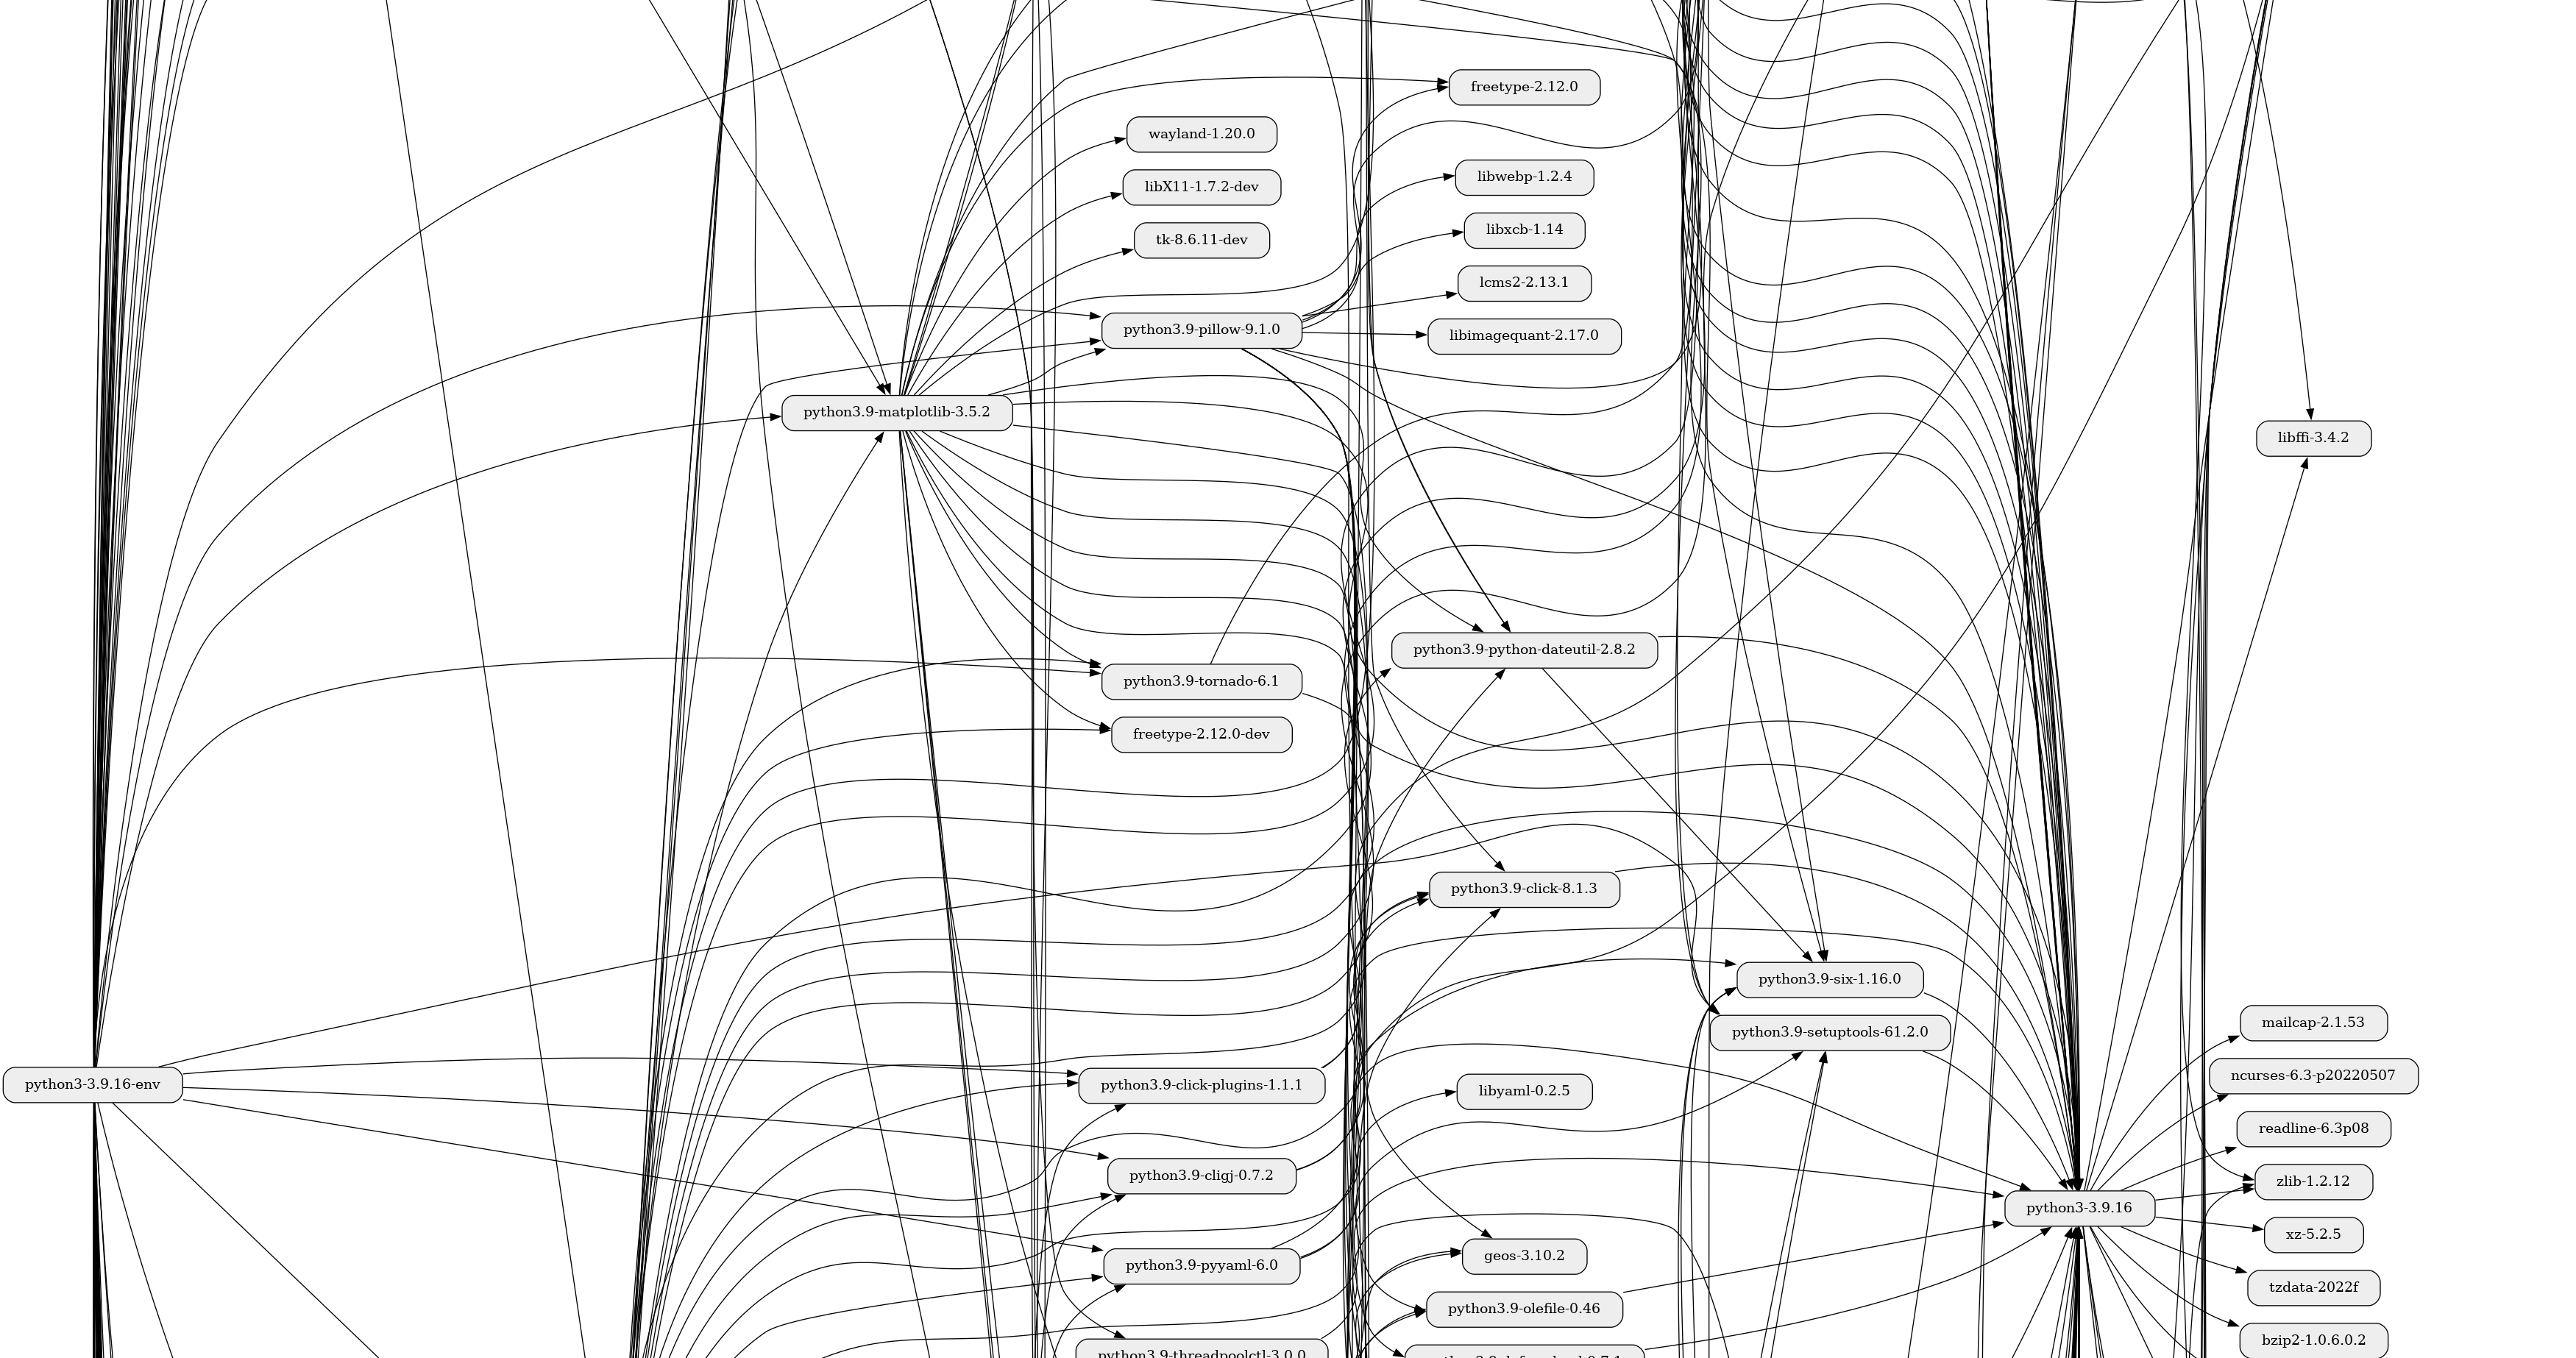
\includegraphics{./imgs/graph.png}
   \caption{Dependency Graph of Flask Project}
   \label{fig:fig2}
\end{figure}

\hypertarget{nix-ecosystem-and-community}{%
\section{Nix Ecosystem and Community}\label{nix-ecosystem-and-community}}

\hypertarget{overview-of-the-nix-ecosystem}{%
\subsection{Overview of the Nix ecosystem}\label{overview-of-the-nix-ecosystem}}

The Nix ecosystem is a collection of tools and utilities that provide a complete solution for creating and managing reproducible software environments. At its core, Nix is a package manager that is designed to provide a reliable, deterministic way of installing and managing software dependencies. Unlike traditional package managers, Nix is designed to work across multiple platforms and with multiple versions of the same software, which makes it particularly well-suited for scientific computing and other research applications.

In addition to the package manager, the Nix ecosystem includes a number of related tools and utilities that can be used to build, deploy, and manage software environments. These tools include:

\begin{itemize}
\item
  Nixpkgs: a collection of over 50,000 pre-built packages that can be easily installed using the Nix package manager.
\item
  NixOS: a Linux distribution based on Nix that provides a complete operating system environment that is fully reproducible and easy to deploy.
\item
  NixOps: a tool for deploying and managing Nix-based software environments in the cloud.
\item
  Lorri: a tool for quickly iterating on Nix-based development environments.
\item
  Hydra: a continuous integration and deployment tool that can be used to build and test Nix packages.
\end{itemize}

Taken together, these tools provide a powerful and flexible set of tools for creating and managing reproducible software environments. Whether you are working on a small research project or a large-scale scientific computing application, the Nix ecosystem provides the tools you need to ensure that your software environment is always reliable, reproducible, and up-to-date.

\hypertarget{community-support-and-resources}{%
\subsection{Community support and resources}\label{community-support-and-resources}}

One of the main advantages when using the nix ecosystem to deploy software is the
community support. The nix community website, which provides a comprehensive
documentation for Nix, including tutorials, guides, and reference manuals.
The community also maintains a package repository, called nixpkgs, which contains
a large number of pre-built packages that can be easily installed using the nix
package manager.

The NixOS community provides various resources for users to get help and support,
including the official forum, Discourse. In my experience, Discourse has been a
great resource for troubleshooting and finding answers to specific questions
related to Nix and its ecosystem.

For example, I recently asked a question on Discourse regarding the installation
of several Python packages, including \texttt{cartopy}, \texttt{cmaps}, \texttt{geocat.viz}, and \texttt{metpy},
for a scientific computing project. Within a few hours, I received a response from
a community member who fixed a build issue in the cartopy package by fixing the
build issue in a pull request. Now the package installs perfectly using the nix package manager.

This kind of community support can be invaluable, especially for users who are new to the Nix ecosystem and may need guidance on how to navigate the various tools and features available. It also shows how active and helpful the NixOS community is, which can be reassuring for users who are considering adopting Nix for their own projects. Overall, the community support and resources available for Nix make it a powerful tool for reproducible scientific computing.

\hypertarget{conclusion}{%
\section{Conclusion}\label{conclusion}}

Nix provides a powerful package management system for scientific computing that can help solve many of the challenges associated with managing software dependencies and versions. Its reproducible builds and declarative package specifications make it ideal for creating consistent and isolated environments for scientific computing. Additionally, the community-driven approach to package maintenance and support ensures that many popular scientific software packages are available in the Nix ecosystem.

While there may be some disadvantages to using Nix, such as limited support for certain niche scientific software packages or the need to work around module systems on HPCs, the benefits of using Nix generally outweigh these challenges. As the scientific computing community continues to adopt and contribute to Nix, we can expect to see even greater support and functionality for scientific software in the future.

\hypertarget{acknowledgment}{%
\section{Acknowledgment}\label{acknowledgment}}

I would like to express my sincere gratitude to Professor Clay Tabor for his invaluable guidance, support, and encouragement throughout my research project. His expertise in scientific computing and his thoughtful insights have been instrumental in shaping this paper. I am also grateful for his patience and willingness to share his time and knowledge with me. Without his guidance, this paper would not have been possible.

I would also like to express my gratitude to the NixOS community and the Nix development team for their invaluable support and assistance during this research project. Their guidance and feedback have been instrumental in shaping my understanding of Nix and its role in creating reproducible environments for scientific computing.

\hypertarget{references}{%
\section*{References}\label{references}}
\addcontentsline{toc}{section}{References}

\hypertarget{refs}{}
\begin{CSLReferences}{1}{0}
\leavevmode\vadjust pre{\hypertarget{ref-bzeznik2017nix}{}}%
Bzeznik, Bruno, Oliver Henriot, Valentin Reis, Olivier Richard, and Laure Tavard. 2017. {``Nix as HPC Package Management System.''} In \emph{Proceedings of the Fourth International Workshop on HPC User Support Tools}, 1--6.

\leavevmode\vadjust pre{\hypertarget{ref-devresse2015nix}{}}%
Devresse, Adrien, Fabien Delalondre, and Felix Schürmann. 2015. {``Nix Based Fully Automated Workflows and Ecosystem to Guarantee Scientific Result Reproducibility Across Software Environments and Systems.''} In \emph{Proceedings of the 3rd International Workshop on Software Engineering for High Performance Computing in Computational Science and Engineering}, 25--31.

\leavevmode\vadjust pre{\hypertarget{ref-dolstra2004nix}{}}%
Dolstra, Eelco, Merijn De Jonge, Eelco Visser, et al. 2004. {``Nix: A Safe and Policy-Free System for Software Deployment.''} In \emph{LISA}, 4:79--92.

\leavevmode\vadjust pre{\hypertarget{ref-reproduce0}{}}%
Ivie, Peter, and Douglas Thain. 2018. {``Reproducibility in Scientific Computing.''} \emph{ACM Computing Surveys (CSUR)} 51 (3): 1--36.

\end{CSLReferences}

\end{document}
